
\usetikzlibrary{arrows}
\usetikzlibrary{arrows.meta}
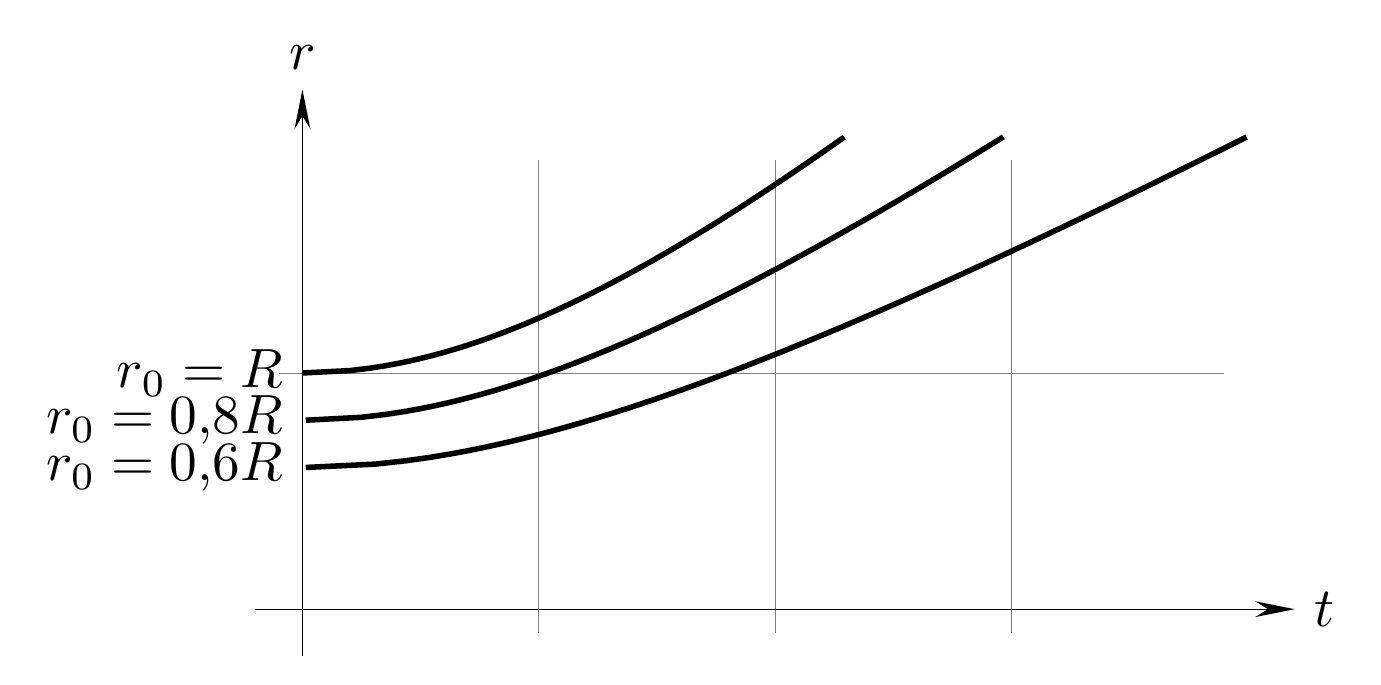
\begin{tikzpicture}[
	domain=0:2,
	declare function={
		time(\x)= (\x > 1) ? sqrt(\x)*sqrt(abs(\x - 1))  + 
		ln( abs( sqrt(\x) + sqrt(abs(\x -1)) ) ) : 0;
	},
	scale=3,
	every node/.style={scale=2}
]
%/*

\draw[very thin,color=gray] (-0.1,-0.1) grid (3.9,1.9);
\draw[-{Stealth[length=5mm, width=2mm]}] (-0.2,0) -- (4.2,0) node[right] {$t$};
\draw[-{Stealth[length=5mm, width=2mm]}] (0, -0.2) -- (0,2.2) node[above] {$r$};
\draw[color=black,samples=100, line width = 2pt, domain=1:2] plot ({time(\x/1)}, \x);
\draw[color=black,samples=100, line width = 2pt, domain=0.8:2] plot ({time(\x/0.8)}, \x);
\draw[color=black,samples=100, line width = 2pt, domain=0.6:2] plot ({time(\x/0.6)}, \x);


\draw (0, 1) node[left]{$r_0 = R$};
\draw (0, 0.8) node[left]{$r_0 = 0{,}8R$};
\draw (0, 0.6) node[left]{$r_0 = 0{,}6R$};
%*/
\end{tikzpicture}
    